\documentclass[a4paper,11pt]{article}
\usepackage{amsmath}
\usepackage{wrapfig}
\usepackage{fancyhdr}
\usepackage{graphicx}
\usepackage{url}
\usepackage{float}
\usepackage{amsmath}
\usepackage{amssymb}
\usepackage[margin=1in]{geometry}

\setlength{\voffset}{-0.5in}
\setlength{\headsep}{5pt}
\newcommand{\suchthat}{\;\ifnum\currentgrouptype=16 \middle\fi|\;}


%===========---------================
% Author John H Allard
% HW Assignment #2
% CMPE 16 - Discrete Math
% October 12th 2014
%===========---------================


\title{ CMPE 16 Homework \# 2}
\author{John Allard, id:1437547}
\date{October 12th, 2014}

\begin{document}
\maketitle

%***************************************
%*********** HomeWork Problems *********
%************** Ten Total **************

\begin{enumerate}


%*******************************
%******** Problem # 1 ************
%*******************************
\item \emph{Give the set represented by each of the expressions below where  $A_1 = \{ \square, 2, 8, a, g \}$,
$A_2 = \{\triangle, -2, 8, a\}$, $A_3 = \{\square, 12, 7, a, g\}$, and $A_4 = \{\square,\triangle,  2, 7, a, b, g\}$. List each element in the set only once (i.e. $\{1, 2\}$ instead of $\{1, 2, 2 \}$).}

  \begin{enumerate}
  \item $A_1 \cup A_2$ \\
  \textbf{Answer :} $A_1 \cup A_2 = \{\square, 2, 8, a, g, -2, \triangle \}$
  \item $A_3 \cap A_4$ \\
  \textbf{Answer :} $A_3 \cap A_4 = \{\square, a, 7, g \}$
  \item $A_4 - A_1$ \\
  \textbf{Answer :} $A_4 - A_1 = \{ \triangle, 7, b \}$
  \item $A_1 - A_4$ \\
  \textbf{Answer :} $A_1 - A_4 = \{ 8 \}$
  \item $\bigcup_{i=1}^{4} A_i$ \\
  \textbf{Answer :} $\bigcup_{i=1}^{4} A_i = \{ \square, 2, 8, a, g, \triangle, -2, 12, b  \}$
  \item $\bigcap_{i=1}^{4} A_i$ \\
  \textbf{Answer :} $\bigcap_{i=1}^{4} A_i = \{ a  \}$
  \end{enumerate}


%*******************************
%******** Problem # 2 ************
%*******************************

\item \emph{For each of the sets below fill in the corresponding regions of a general Venn diagram for
3 sets. (The Venn diagram should have 3 sets in each case.)}
 \textbf{Answers on last page.}
  \begin{enumerate}
  \item $A \cup \overline{B} \cup C$ 
  \item $C - ( A \cap B)$
  \item $\overline{(B - C) \cup A} $
  \end{enumerate}


%*******************************
%******** Problem # 3************
%*******************************

\item \emph{Write $ \bigcup_{i\in \mathbb{Z}} (i, i+1)$ as the difference of two well known sets. Here $(i, i+1)$ is the open interval of the real line with endpoints $i$ and $i + 1$. (That is, $(i, i + 1) = {x \in \mathbb{R} : i < x < i + 1}$).} \\ \\
\textbf{Answer :} The set $Y = \bigcup_{i\in \mathbb{Z}} (i, i+1)$ can be written as the difference of $\mathbb{R}$ and $\mathbb{N}$ ; $Y = \mathbb{R}-\mathbb{N} $. This is because $Y$ includes all numbers in $\mathbb{R}$ up-to but not including the actual integer values in $\mathbb{Z}$


%*******************************
%******** Problem # 4************
%*******************************

\item Using only the symbols 4, Z, S, P, W, $\emptyset, \subseteq, \in, \cup, \cap,$ -, =, \{, \}, ),(, and $\neq$, express the following
statements
  
  \begin{enumerate}
  	\item 4 is pale and shy \\
  	\textbf{Answer :} $4 \in (P \cap S)$
  	\item All worried integers are pale. \\
  	\textbf{Answer :} $W \subseteq P$
  	\item Every integer is shy, worried, or pale. \\
  	\textbf{Answer :} $\mathbb{Z} \subseteq (P \cup S \cup W)$
  	\item There are worried integers that are not shy. \\
  	\textbf{Answer :} $(W - S) \neq \emptyset$
  \end{enumerate}


%*******************************
%******** Problem # 5************
%*******************************

\item Let P and Q be the statements \\ P I eat garlic. \\ Q I go to the dentist. \\
Rewrite each of the statements below using P and Q and logical connectives $(\neg, \wedge, \vee, \implies)$.

  \begin{enumerate}
  \item I don't eat Garlic \\
  \textbf{Answer :} $ \neg P$
  \item I don't go to the Dentist, but I eat garlic. \\
  \textbf{Answer :} $ \neg Q \wedge P$
  \item I eat garlic or I don't go to the dentist. \\
  \textbf{Answer :} $P \vee \neg Q$
  \item Whenever I go to the dentist, I don't eat garlic. \\
  \textbf{Answer :} $ Q \implies \neg P$
  \end{enumerate}

%*******************************
%******** Problem # 6************
%*******************************
\item Let P, Q and R be the statements \\ P I use plastic bags. \\ Q I use paper bags. \\ R I help the environment.

  \begin{enumerate}
  \item $ \neg P$
  \item $P \wedge Q$
  \item $Q \implies \neg R$
  \item $\neg (P \implies R)$
  \end{enumerate}

%*******************************
%******** Problem # 7 ************
%*******************************
\item Use a truth table to determine the values of each of the logical expressions below. Both of
your truth tables should have at least 3 intermediate columns.
  \begin{enumerate}
  \item $\neg (P \vee Q) \wedge \neg Q$
  \item $ (P \vee Q) \wedge (Q \vee R) \wedge \neg (P \wedge R)$
  \end{enumerate}


%*******************************
%******** Problem # 8 ************
%*******************************
\item Convert each of the following statements into the form “If P then Q” without changing
their meanings. (Some of these statements might not be True and that’s okay.)
  \begin{enumerate}
  \item
  \end{enumerate}


%*******************************
%******** Problem # 9 ************
%*******************************
\item As discussed in class, given a finite set S of size n and an ordering s1, s2, . . . , sn of the n
elements in S, we can represent the subsets of S using bit vectors of length n ({0, 1}
n). For a subset
A ⊆ S, the corresponding bit vector b(A) = (b1, b2, . . . , bn) where bi = 1 if si ∈ A and bi = 0 if si 6∈ A.
Let S be the elements from the four sets in Problem 1 ordered as , 4, −2, 2, 7, 8, 12, a, b, g.
  \begin{enumerate}
  \item
  \end{enumerate}



%*******************************
%******** Problem # 10 ************
%*******************************
\item Given the bit vectors b(B) = (b1, b2, . . . , bn) and b(D) = (d1, d2, . . . , dn) representing two
subsets B and D. In each case below explain how you would calculate the required bit vector (in
general), and then apply your method to obtain the result for B = A1 and D = A4 from Problem 1.
  \begin{enumerate}
  \item
  \end{enumerate}

\end{enumerate}

  \begin{wrapfigure}{r}{1.0\textwidth}
     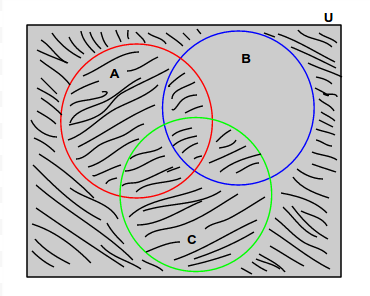
\includegraphics[width=4.4in]{2Avenn}
   \caption{Venn Diagram for Problem 2a}
   \label{fig:tutorial}
  \end{wrapfigure} 

    \begin{wrapfigure}{r}{1.0\textwidth}
     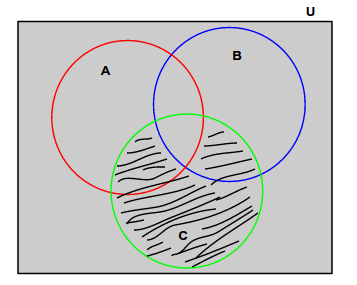
\includegraphics[width=4.4in]{2Bvenn}
   \caption{Venn Diagram for Problem 2b}
   \label{fig:tutorial}
  \end{wrapfigure} 

    \begin{wrapfigure}{r}{1.0\textwidth}
     \includegraphics[width=4.4in]{2Cvenn}
   \caption{Venn Diagram for Problem 2c}
   \label{fig:tutorial}
  \end{wrapfigure} 



\end{document}